\startchapter{Mixture of Realistic Molecules} \label{ch:5}
\section{Description}

In Chapter \ref{ch:4}, test cases indicate that for one type of molecule at surfaces, even combining the information of all the three spectral information, the built LP instances are not sufficient to obtain the target composition in most test cases. In another word, the existing spectral information is not adequate to obtain the target composition for one type of molecule at surfaces. Multiple return compositions can build the target spectra. Besides one type of molecule at surfaces, we are also interested in the case where candidates coming from different molecules. For a mixture of different molecules at surfaces, we want to figure out with available spectral information, can the built LP instances help to return the target composition. In the case where the LP instance is sufficient to obtain the target composition, we are interested in which the specific combination of spectroscopy techniques is adequate. Moreover, we want to know the accuracy of this specific combination in obtaining the target composition. \\

\section{Test Cases}
The first part of this section, we study the test cases where each molecule's candidates expanded in $[0^{\circ}, 90^{\circ})$ on $\theta$, to see which spectral information is sufficient in obtaining the target composition. Then in the second part, we study the cases where each molecule's candidates expanded in $[0^{\circ}, 180^{\circ}]$ on $\theta$. \\

\subsection{Test Cases Considering Candidates of Each Amino Acid Expanded in $[0^{\circ}$, $90^{\circ})$ on $\theta$ in a Mixture of Amino Acids} \label{testcase51}
To study the molecular orientation distribution of various molecules at surfaces, further test cases are constructed. These test cases have the following common settings. \\

First, as mentioned in Chapter \ref{ch:1}, there are six different amino acids in the mixture: Met, Leu, Ile, Ala, Thr and Val. For each amino acid, only the difference of $\theta$ is considered. Each amino acid has nine candidates in the mixture. They have the following $\theta$ values: $0^{\circ}$,  $10^{\circ}$, $20^{\circ}$, $30^{\circ}$, $40^{\circ}$, $50^{\circ}$, $60^{\circ}$, $70^{\circ}$ and $80^{\circ}$. When $\theta$ equals $90^{\circ}$, the SFG spectra has zero intensity. Therefore the corresponding candidate is excluded from all the test cases. As a result, there are 54 candidates in the mixture. \\

Second, the target composition needs to be generated. The operation includes two steps: randomly pick one candidate from each of the amino acid's nine candidates, then randomly generate a percentage for the selected candidate. The target composition is made of six randomly selected candidates with assigned percentage coming from the amino acids. The remaining $48$ candidates have $0$ percentage in the target composition. That is six selected candidate makes 100\% component of the mixture. \\

Third, the IR, Raman and SFG spectra need to be generated for all $54$ candidates and the target. \\

Table \ref{tab:5.1} displays a set of test cases. Each test case contains different spectral information. In Case 1, candidates $x$- and $z$-polarized IR spectra are obtained. The target's IR spectra are generated by the dot product of the target composition and all the candidates' spectral data. Then the corresponding LP instance is conducted using Equation \ref{eq:3.4}. Therefore, we conclude that in Case 1, only IR information is used to build the LP instance. Similarly, in Case 2, only Raman spectral information is used to build the LP instance. In Case 3, only SFG spectral information is used to build the LP instance. \\

\begin{table}[ht!]
\begin{center}
{\def\arraystretch{1.5}
\begin{tabular}{| l | p{3in} | }
\hline
Test Case & Spectral Information \\
\hline
Case 1 & $x$ and $z$ polarized IR spectra\\
\hline
Case 2 & $xx$, $xy$, $xz$ and $zz$ polarized Raman spectra \\
\hline
Case 3 & $xxz$, $xzx$ and $zzz$ polarized SFG spectra \\
\hline
Case 4 & $x$ and $z$ polarized IR spectra \newline $xx$, $xy$, $xz$ and $zz$ polarized Raman spectra \\
\hline
Case 5 & $x$ and $z$ polarized IR spectra \newline $xxz$, $xzx$ and $zzz$ polarized SFG spectra \\
\hline
Case 6 & $xx$, $xy$, $xz$ and $zz$ polarized Raman spectra \newline $xxz$, $xzx$ and $zzz$ polarized SFG spectra \\
\hline
Case 7 & $x$ and $z$ polarized IR spectra \newline
 $xx$, $xy$, $xz$ and $zz$ polarized Raman spectra \newline 
 $xx$, $xzx$ and $zzz$ polarized SFG spectra \\
\hline
\end{tabular} 
}
\end{center}
\caption{Detailed test cases set for the mixture of amino acids.} 
\label{tab:5.1} 
\end{table}	

Starting from Case 4, spectral information of different spectroscopy techniques are combined to build the LP instance. In Case 4, IR spectral information is combined with Raman. In Case 5, IR spectral information is combined with SFG. In Case 6, Raman and SFG spectral information are incorporated. At the end, in Case 7, information of all three spectral is put together: IR, Raman and SFG. \\

Finally, this set of test cases is run 100 times in order to see which test case in the set returns the target composition with the highest accuracy. This accuracy is measured by the time of the LP solver returns the target composition. The scoring mechanism that measures whether or not a return composition matches the target one is described in the next section. \\

\subsection{Scoring method}

At the first glance, it may appear a useful approach that the sum of residuals between the spectra composed by the return composition and the target one can be used to measure the accuracy of the return composition. However, recall that in most test cases conducted earlier, the spectra generated by the return composition are identical to the target ones. The sum of residuals between these spectra is negligible, which makes it appropriate to use it as a scoring criterion. \\

Another way to measure the accuracy of the return composition is to compare it directly with the target composition. Calculating the sum of the residuals between a target composition and a return one directly can be a fast approach to evaluate the accuracy of each test case. The shortage of this approach is that it cannot be used to measure in realistic test cases where the target composition is unknown. However, in the current test cases, this approach can be a way to evaluate the return composition for all the test cases where the target compositions are known in advance. \\

The return composition of each test case in the set is obtained for each run. Each return composition is compared with the target one to calculate the sum of the residuals. If the sum is smaller than a certain threshold, which is $10^{-7}$, then the return composition is considered to be the same as the target one. \\

\begin{table}[ht!]
\begin{center}
{\def\arraystretch{1.5}
\begin{tabular}{| l | l | l | l | l | l | l | l |}
\hline
Test Case & 1 & 2 & 3 & 4 & 5 & 6 & 7 \\ \hline
\# of Returning Target Composition& 0 & 100 & 100 & 100 & 100 & 100 & 100 \\ \hline
\end{tabular} 
}
\end{center}
\caption{Result analysis for test cases considering a mixture of amino acids with candidates expanded in $[0^{\circ}, 90^{\circ})$ on $\theta$ for each amino acid. \# of returning target composition indicates how many times each test case in the set return a composition that matches the target one.}
\label{tab:5.2}
\end{table}	

%\begin{figure}[!ht]
%\centering
%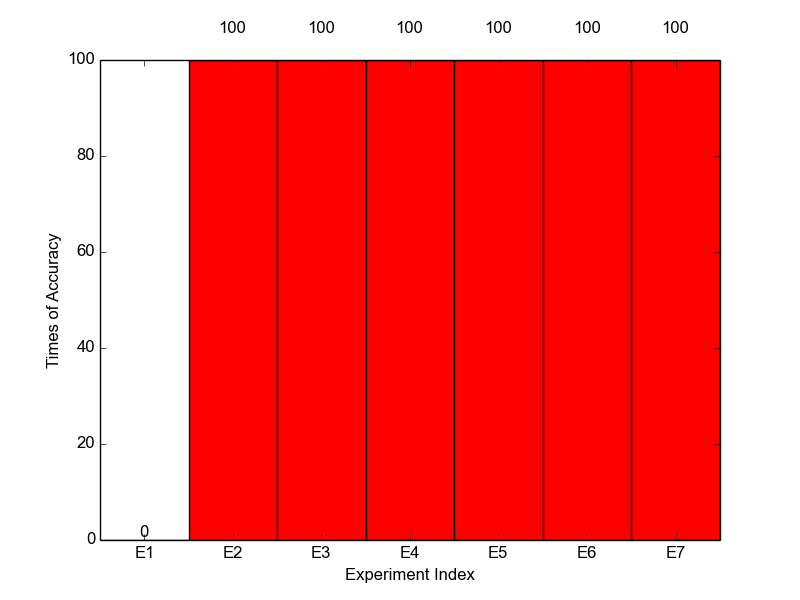
\includegraphics[scale=0.7]{Figures/accuracy_pecent_result8_mixture.png}
%\caption{Accuracy analysis for test cases considering a mixture of amino acids with candidates from $0^{\circ}$ to $80^{\circ}$ on $\theta$ for each amino acid. Accuracy indicates how many times each test case in the set return a composition that matches the target one.}  \label{fig:5.1}
%\end{figure}

The test case set is run 100 times, based on the scoring method, the result is shown in 
Table \ref{tab:5.2}. Cases 2, 3, 4, 5, 6 and 7 return the target composition in all 100 runs. This result indicates that Raman or SFG alone is sufficient to obtain the target composition, for a mixture of amino acids with candidates expanded in $[0^{\circ}, 90^{\circ})$ on $\theta$ for each amino acid. Any test cases that contain Raman and SFG spectral information result in the same accuracy. \\

The only exception is Case 1. The accuracy is fairly low, which indicates that IR spectra alone do not contain sufficient information in order to obtain the target composition. \\

To gain more understanding of the return composition of Case 1, the test case set is re-run 100 times. In each run, IR $x$- and $z$-polarized spectra are plotted both by the returned composition and the target one. The result is that these spectra conducted by the two different compositions are identical in each run. Let us randomly take one run as an example. Figure \ref{fig:5.1} displays the plotted spectra. Note that they are identical to each other. The residual is very small for the data points where these two spectra are not overlapped. This further indicates that IR spectral information is not sufficient to obtain the target composition.\\

%(TODO: rewrite or remove this paragraph) Comparatively, SFG has three unique polarizations, and Raman has four unique polarizations. From each projection's spectrum, we evenly select 200 data points. This means that one more projection will bring in 200 more constraints or 400 more (when we take the absolute sign off) constraints to the LP model. This would make a huge difference in the LP model, in term of further refining the candidate selection in target composition. However, it is still too early for us to say that Raman has more orientation information because it has four unique polarizations. Because for Raman's any polarization, the spectrum of candidate with $\theta$ equals to one degree is identical to the one of candidate with this $\theta$ degree's complementary. For example, the Raman spectra for candidate with $\theta$ of $10^{\circ}$, is the same as candidate with $\theta$ of $170^{\circ}$. And for IR, it is the same case. Only SFG tells the differences between these two degrees, as the spectra for candidate with $\theta$ of one degree is symmetric to its complementary along wavenumber as shown in Figure \ref{fig:5.8}. \\

\begin{figure}[!ht] 
\centering
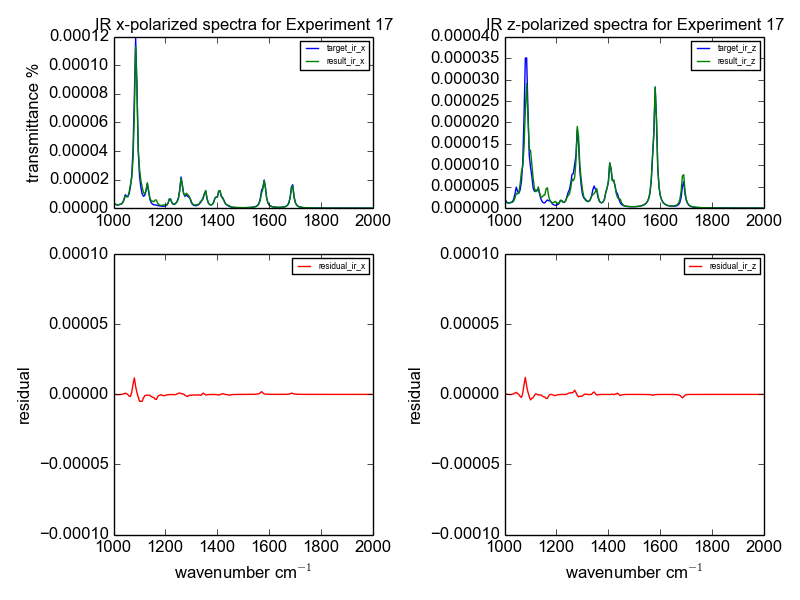
\includegraphics[scale=0.7]{Figures/chapter5_result_target_residual_plotting__ir_result8_run1.png}
\caption{IR spectra plotted by the result composition and the target composition of one ramdon run when considering each amino acid candidates expanded in $[0^{\circ}, 90^{\circ})$ on $\theta$ in a mixture of realistic molecules.} \label{fig:5.1}
\end{figure}

\subsection{Test Cases Considering Candidates of Each Amino Acid candidates Expanded in $[0^{\circ}$,$180^{\circ}]$ on $\theta$ in a Mixture of Amino Acids}
To further study the capacity of the LP models, the candidate pool is expanded in $[0^{\circ}, 180^{\circ}]$ in terms of the $\theta$ value, excluding $90^{\circ}$. Therefore, each amino acid has $18$ candidates. In total, there are $108$ candidates in the mixture. The same set of test cases as in Table \ref{tab:5.1} is used. The only difference is that instead of randomly selecting one candidate from nine candidates, it is selected from eighteen. All $108$ candidates' IR, Raman and SFG spectra need to be generated. Table \ref{tab:5.3} illustrates the results obtained in $100$ runs. The accuracy in Case 1 is still low. This is not surprising as the complexity of the candidates has increased. Moreover, IR spectra for candidate of $\theta$ is identical to $180^{\circ}-\theta$, as shown in Figure \ref{fig:A.1}. This also increases the difficulty for the LP solver to return the target composition. \\

%\begin{figure}[!ht]
%\centering
%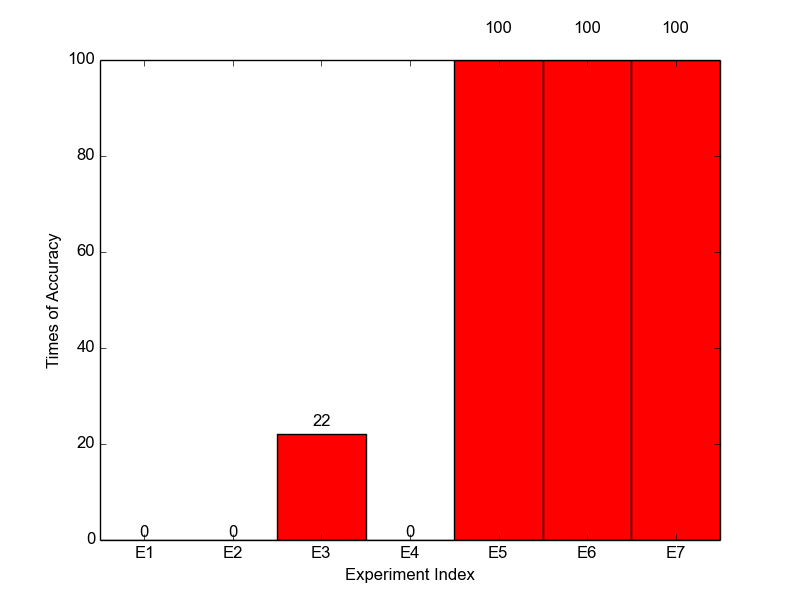
\includegraphics[scale=0.7]{Figures/accuracy_pecent_result10_mixture.png}
%\caption{Accuracy analysis for test cases considering a mixture of amino acids with candidates from $0^{\circ}$ to $180^{\circ}$ on $\theta$ for each amino acid. Accuracy indicates how many times each test case in the set return a composition matches the target one.} \label{fig:5.3}
%\end{figure}

\begin{table}[ht!]
\begin{center}
{\def\arraystretch{1.5}
\begin{tabular}{| l | l | l | l | l | l | l | l |}
\hline
Test Case & 1 & 2 & 3 & 4 & 5 & 6 & 7 \\ \hline
\# of Returning Target Composition& 0 & 0 & 22 & 0 & 100 & 100 & 100 \\ \hline
\end{tabular} 
}
\end{center}
\caption{Result analysis for test cases considering a mixture of amino acids with candidates expanded in $[0^{\circ}, 180^{\circ}]$ on $\theta$ for each amino acid, excluding $90^{\circ}$. \# of returning target composition indicates how many times each test case in the set return a composition that matches the target one.}
\label{tab:5.3}
\end{table}	

However, it should be noted that the accuracy for Case 2 has dramatically dropped. This can be caused by the fact that the Raman spectra for one candidate with a $\theta$ is identical to $180^{\circ}-\theta$ as displayed in Figure \ref{fig:A.2}. \\

Table \ref{tab:5.3} shows that the accuracy for Case 3 is no longer high. After increasing the number of amino acid candidates from nine to eighteen, the complexity of candidates has increased as well. SFG spectra for candidate of $\theta$ is symmetric to $180^{\circ}-\theta$, which has increased the difference of the candidates as shown in Figure \ref{fig:A.3}. However, the SFG spectral information is still not sufficient for obtaining the target composition. \\

The number of returning the target composition increases when using the combinations of IR and SFG or Raman and SFG. Table \ref{tab:5.3} shows that Cases 5, 6, and 7 all have 100\% accuracies. SFG spectra is needed as it is the only information that distinguish candidate of $\theta$ from candidate of $180^{\circ}-\theta$. Once combining SFG spectral information with other technique to obtain extra spectral information, it is sufficient to obtain the target composition. \\

Although the accuracy in Case 2 is low, there is still some noticable result in the return composition: for each amino acid, the percentage assigned is correct; however, the candidate presented may not always be correct. We observe that it is either the correct $\theta$, or $180^{\circ}-\theta$. We randomly select one run of the test case set as an example, Figure \ref{fig:5.4} displays the target composition. Figure \ref{fig:5.5} displays the return composition of Case 2. Figure \ref{fig:5.6} is the return composition of Case 6. Figure \ref{fig:5.4} and \ref{fig:5.6} are identical, which means the return composition of Case 6 is the same as the target one. The values in Figure \ref{fig:5.5} are the same as Figure \ref{fig:5.4}. However, the position of each value is not the same in two the figures. For example, the percentage value $0.30$ of Met is for $\theta = 120^{\circ}$ in Figure \ref{fig:5.4}, but is for $\theta = 60^{\circ}$ in Figure \ref{fig:5.5}. These two angles are complementary. This observation is the same for Ile, Ala, Thr, and Val in the figures. This observation is a general case across all the runs of the test case set. The return composition of Case 6 matches the target one. However, the return composition of Case 2 fails to pick the correct candidate of each amino acid from $\theta$ and $180^{\circ}-\theta$. This can be explained as the Raman spectra for a specific value of $\theta$ is the same as the one of $180^{\circ}-\theta$. \\

\begin{figure}[!ht] 
\centering
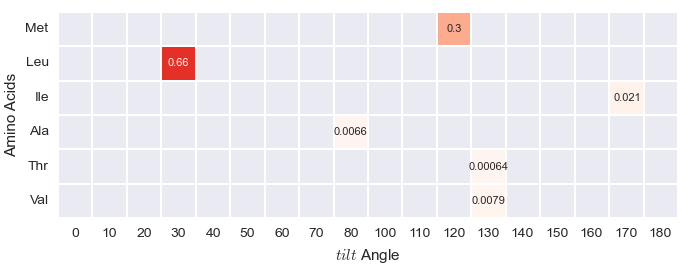
\includegraphics[scale=0.7]{Figures/mixture_target_composition_for_one_run_theta_0_180.png}
\caption{Target composition of one random run of six mixed amino acids with candidates expanded in $[0^{\circ}, 180^{\circ}]$ on $\theta$ for each amino acid, excluding $90^{\circ}$. More detailed data of this target composition can be found in Appendix \ref{eqn:A.1}. } 
\label{fig:5.4}
\end{figure}

\begin{figure}[!ht] 
\centering
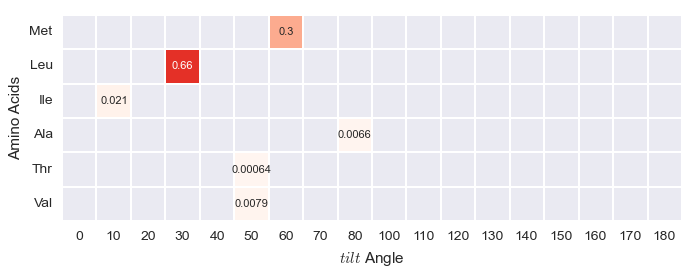
\includegraphics[scale=0.7]{Figures/mixture_return_composition_of_E2_for_one_run_theta_0_180.png}
\caption{Return composition of Case 2 for one random run of six mixed amino acids with candidates expanded in $[0^{\circ}, 180^{\circ}]$ on $\theta$, excluding $90^{\circ}$. More detailed data of this return composition can be found in Appendix \ref{eqn:A.2}.} 
\label{fig:5.5}
\end{figure}

\begin{figure}[!ht] 
\centering
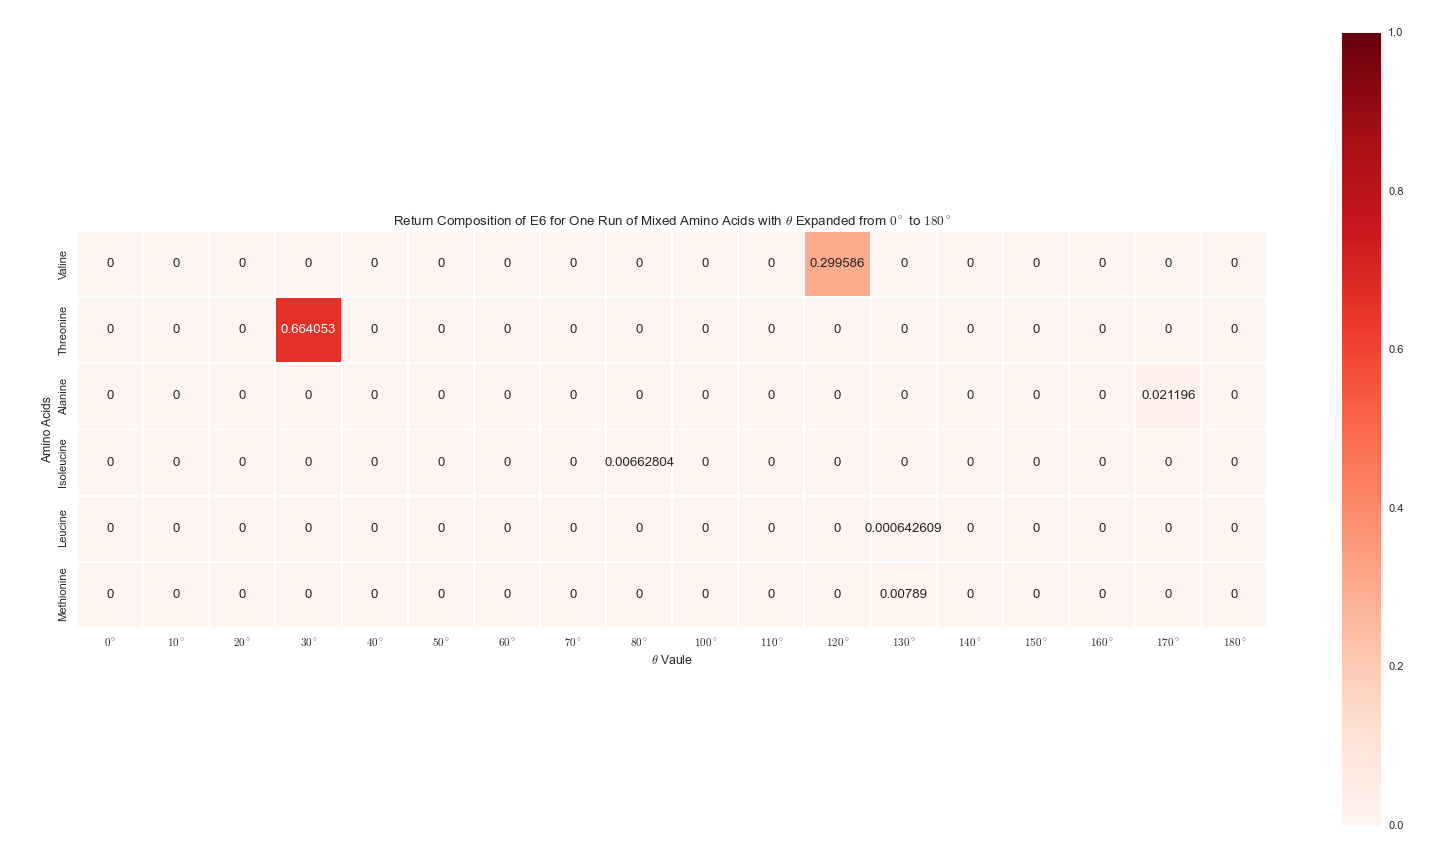
\includegraphics[scale=0.7]{Figures/mixture_return_composition_of_E6_for_one_run_theta_0_180.png}
\caption{Return composition of Case 6 for one random run of six mixed amino acids with candidates expanded in $[0^{\circ}, 180^{\circ}]$ on $\theta$, excluding $90^{\circ}$. More detailed data of this return composition can be found in Appendix \ref{eqn:A.3}.} 
\label{fig:5.6}
\end{figure}

\section{Conclusion}
Raman or SFG spectral information alone is sufficient to obtain the target composition, when considering a mixture of molecules with candidates expanded in $[0^{\circ}, 90^{\circ})$ on $\theta$ for each amino acid. When the candidates of each molecule are expanded in $[0^{\circ}, 180^{\circ}]$ on $\theta$, excluding $90^{\circ}$, SFG spectral information needs to be combined with IR or Raman in order to obtain the target composition. SFG spectral information is needed, as it is the only information to distinguish candidate of $\theta$ from the one of $180^{\circ}-\theta$.\\
